% RL-Augmented Smart Contract Auditing: Presentation 1
% Minimalist Beamer Theme
\documentclass[aspectratio=169]{beamer}

% Theme Configuration - Minimalist
\usetheme{default}
\usecolortheme{dove}
\setbeamertemplate{navigation symbols}{}
\setbeamertemplate{footline}[frame number]
\setbeamertemplate{itemize items}[circle]
\setbeamercolor{title}{fg=black}
\setbeamercolor{frametitle}{fg=black}
\setbeamerfont{title}{size=\Large,series=\bfseries}
\setbeamerfont{frametitle}{size=\large,series=\bfseries}

% Packages
\usepackage{graphicx}
\usepackage{tikz}
\usetikzlibrary{shapes,arrows,positioning,fit,backgrounds}
\usepackage{amsmath}
\usepackage{amssymb}
\usepackage{listings}
\usepackage{xcolor}

% Color Definitions
\definecolor{baseblue}{RGB}{70,130,180}
\definecolor{rlgreen}{RGB}{34,139,34}
\definecolor{costred}{RGB}{220,20,60}
\definecolor{accentorange}{RGB}{255,140,0}

% Title Information
\title{RL-Augmented Smart Contract Auditing}
\subtitle{Adaptive Orchestration for Cost-Efficient Vulnerability Detection}
\author{Research Honors Project}
\date{\today}

\begin{document}

% Title Slide
\begin{frame}
\titlepage
\end{frame}

% Slide 1: Literature Survey
\begin{frame}{Literature Survey}
\frametitle{Base Paper: LLM-SmartAudit}
\framesubtitle{Advanced Smart Contract Vulnerability Detection via LLM-Powered Multi-Agent Systems (IEEE TSE 2025)}

\vspace{0.3cm}

\textbf{Core Contributions:}
\begin{itemize}
    \item Multi-agent framework with specialized roles:
    \begin{itemize}
        \item Project Manager
        \item Smart Contract Auditor
        \item Solidity Programming Expert
        \item Smart Contract Counselor
    \end{itemize}
    \item Two operational modes:
    \begin{itemize}
        \item \textbf{BA} (Broad Analysis) — general vulnerability sweep
        \item \textbf{TA} (Targeted Analysis) — 40 predefined vulnerability scenarios
    \end{itemize}
    \item Achieves \textbf{98\% accuracy} on common vulnerabilities, \textbf{47.6\%} on real-world contracts
\end{itemize}

\vspace{0.3cm}

\textbf{\textcolor{costred}{Identified Gaps:}}
\begin{itemize}
    \item No dynamic/runtime verification
    \item Fixed, hand-authored control flow and stopping criterion
    \item Fixed 40-scenario coverage ceiling
    \item Struggles on novel logic bugs
\end{itemize}

\end{frame}

% Slide 2: Base Architecture
\begin{frame}{Base Architecture: LLM-SmartAudit Agent Flow}
\frametitle{Existing Multi-Agent Conversation System}

\begin{center}
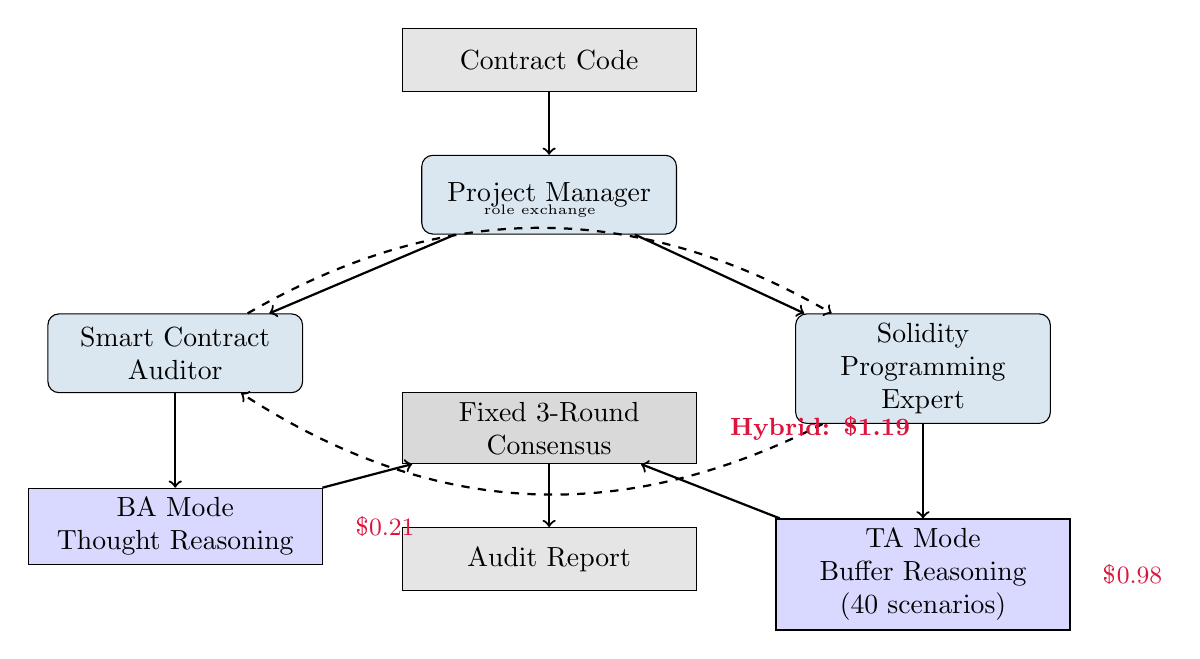
\begin{tikzpicture}[
    node distance=1.5cm,
    agent/.style={rectangle, draw, fill=baseblue!20, text width=3cm, align=center, minimum height=1cm, rounded corners},
    process/.style={rectangle, draw, fill=gray!20, text width=3.5cm, align=center, minimum height=0.8cm},
    decision/.style={diamond, draw, fill=accentorange!20, text width=2cm, align=center, aspect=2},
    arrow/.style={->, thick}
]

% Input
\node[process] (contract) {Contract Code};

% Project Manager
\node[agent, below=0.8cm of contract] (pm) {Project Manager};

% Agents
\node[agent, below left=1cm and 1.5cm of pm] (auditor) {Smart Contract\\Auditor};
\node[agent, below right=1cm and 1.5cm of pm] (expert) {Solidity\\Programming Expert};

% Analysis Modes
\node[process, below=1.2cm of auditor, fill=blue!15] (ba) {BA Mode\\Thought Reasoning};
\node[process, below=1.2cm of expert, fill=blue!15] (ta) {TA Mode\\Buffer Reasoning\\(40 scenarios)};

% Consensus
\node[process, below=2cm of pm, fill=gray!30] (consensus) {Fixed 3-Round\\Consensus};

% Output
\node[process, below=0.8cm of consensus] (report) {Audit Report};

% Arrows
\draw[arrow] (contract) -- (pm);
\draw[arrow] (pm) -- (auditor);
\draw[arrow] (pm) -- (expert);
\draw[arrow] (auditor) -- (ba);
\draw[arrow] (expert) -- (ta);
\draw[arrow] (ba) -- (consensus);
\draw[arrow] (ta) -- (consensus);
\draw[arrow] (consensus) -- (report);

% Role exchange
\draw[arrow, dashed, bend left=30] (auditor) to node[above, sloped, font=\tiny] {role exchange} (expert);
\draw[arrow, dashed, bend left=30] (expert) to (auditor);

% Cost annotation
\node[right=0.3cm of ba, text=costred, font=\small] {\$0.21};
\node[right=0.3cm of ta, text=costred, font=\small] {\$0.98};
\node[right=0.3cm of consensus, text=costred, font=\small\bfseries] {Hybrid: \$1.19};

\end{tikzpicture}
\end{center}

\vspace{0.2cm}
\textbf{Key Issue:} Hybrid mode always runs both BA and TA regardless of contract complexity

\end{frame}

% Slide 3: Existing Work
\begin{frame}{Existing Work: RL-Based Smart Contract Auditor}
\frametitle{Prior Project — Foundation for Current Research}

\begin{columns}[T]
\begin{column}{0.5\textwidth}
\textbf{Architecture:}
\begin{itemize}
    \item Reasoning backbone: Groq-hosted LLaMA 3.3 70B
    \item Trained on SmartBugs Curated dataset
    \item OpenEnv-compatible RL environment
    \item Deployed on HuggingFace Spaces
\end{itemize}

\vspace{0.5cm}

\textbf{Contributions:}
\begin{itemize}
    \item Reusable RL environment scaffolding
    \item Low-cost inference pipeline (Groq)
    \item Proof-of-concept for RL in smart contract auditing
\end{itemize}
\end{column}

\begin{column}{0.5\textwidth}
\begin{center}
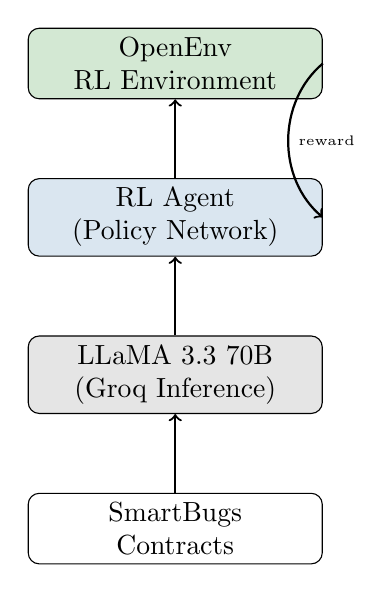
\begin{tikzpicture}[
    node distance=1cm,
    box/.style={rectangle, draw, text width=3.5cm, align=center, minimum height=0.8cm, rounded corners}
]

\node[box, fill=rlgreen!20] (env) {OpenEnv\\RL Environment};
\node[box, below=of env, fill=baseblue!20] (agent) {RL Agent\\(Policy Network)};
\node[box, below=of agent, fill=gray!20] (llm) {LLaMA 3.3 70B\\(Groq Inference)};
\node[box, below=of llm] (contract) {SmartBugs\\Contracts};

\draw[->, thick] (contract) -- (llm);
\draw[->, thick] (llm) -- (agent);
\draw[->, thick] (agent) -- (env);
\draw[->, thick, bend right=50] (env.east) to node[right, font=\tiny] {reward} (agent.east);

\end{tikzpicture}
\end{center}

\vspace{0.3cm}
\textbf{Motivation:} Established scaffolding for current research direction
\end{column}
\end{columns}

\end{frame}

% Slide 4: Proposed Architecture
\begin{frame}{Proposed Architecture: RL Policy Hooked into LLM-SmartAudit}
\frametitle{Learned Adaptive Orchestration Layer}

\begin{center}
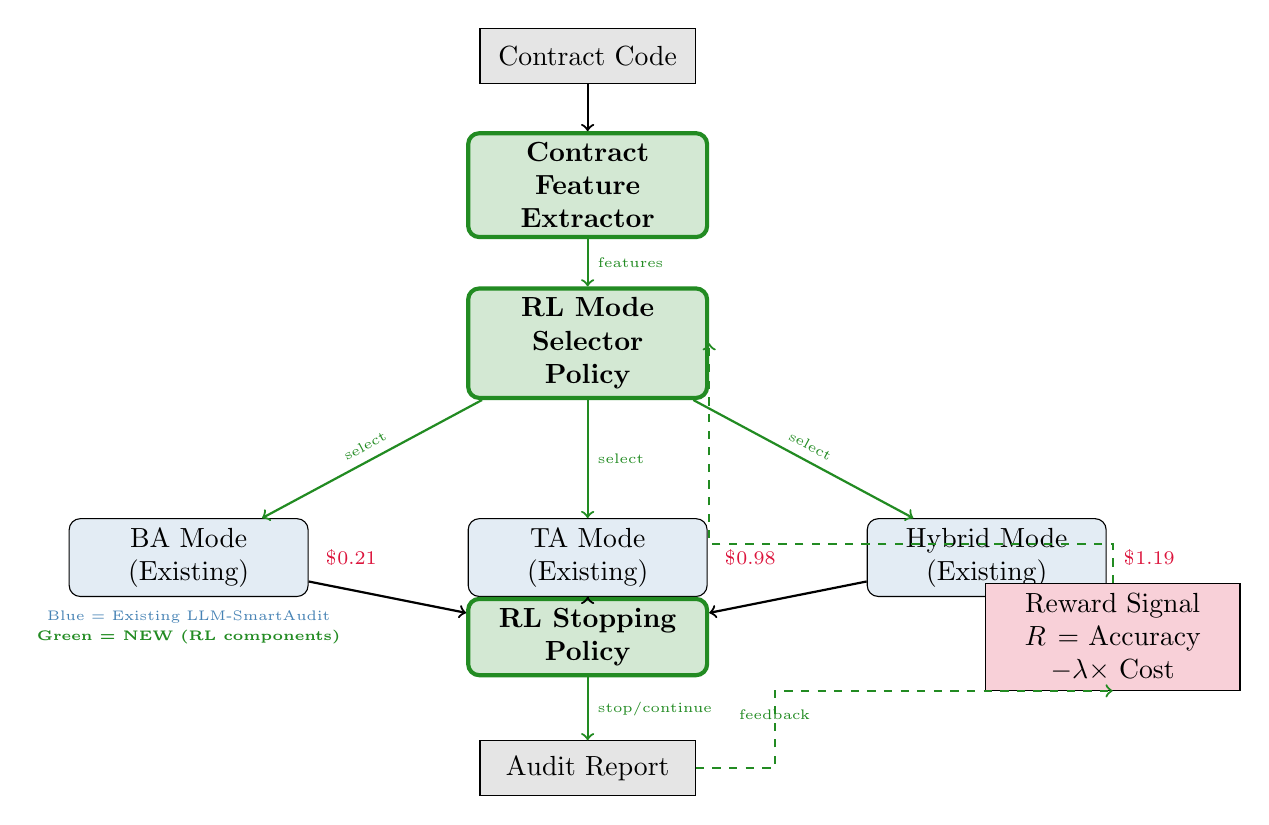
\begin{tikzpicture}[
    node distance=1.2cm,
    newbox/.style={rectangle, draw=rlgreen, line width=1.5pt, fill=rlgreen!20, text width=2.8cm, align=center, minimum height=0.9cm, rounded corners, font=\bfseries},
    oldbox/.style={rectangle, draw, fill=baseblue!15, text width=2.8cm, align=center, minimum height=0.9cm, rounded corners},
    process/.style={rectangle, draw, fill=gray!20, text width=2.5cm, align=center, minimum height=0.7cm},
    arrow/.style={->, thick},
    rlarrow/.style={->, thick, color=rlgreen}
]

% Input layer
\node[process] (contract) {Contract Code};

% Feature extraction (NEW)
\node[newbox, below=0.6cm of contract] (features) {Contract\\Feature Extractor};

% RL Policy (NEW - emphasized)
\node[newbox, below=0.6cm of features, minimum height=1.2cm] (policy) {RL Mode Selector\\Policy};

% Mode branches
\node[oldbox, below left=1.5cm and 2cm of policy] (ba) {BA Mode\\(Existing)};
\node[oldbox, below=1.5cm of policy] (ta) {TA Mode\\(Existing)};
\node[oldbox, below right=1.5cm and 2cm of policy] (hybrid) {Hybrid Mode\\(Existing)};

% Stopping policy (NEW)
\node[newbox, below=2.5cm of policy] (stopping) {RL Stopping\\Policy};

% Output
\node[process, below=0.8cm of stopping] (report) {Audit Report};

% Reward signal
\node[process, right=3.5cm of stopping, fill=costred!20, text width=3cm] (reward) {Reward Signal\\$R = $ Accuracy\\$- \lambda \times$ Cost};

% Arrows
\draw[arrow] (contract) -- (features);
\draw[rlarrow] (features) -- node[right, font=\tiny] {features} (policy);
\draw[rlarrow] (policy) -- node[above, sloped, font=\tiny] {select} (ba);
\draw[rlarrow] (policy) -- node[right, font=\tiny] {select} (ta);
\draw[rlarrow] (policy) -- node[above, sloped, font=\tiny] {select} (hybrid);

\draw[arrow] (ba) -- (stopping);
\draw[arrow] (ta) -- (stopping);
\draw[arrow] (hybrid) -- (stopping);

\draw[rlarrow] (stopping) -- node[right, font=\tiny] {stop/continue} (report);

% Feedback loop
\draw[rlarrow, dashed] (report.east) -- ++(1,0) |- node[above, pos=0.25, font=\tiny] {feedback} (reward.south);
\draw[rlarrow, dashed] (reward.north) -- ++(0,0.5) -| (policy.east);

% Cost annotations
\node[right=0.1cm of ba, text=costred, font=\scriptsize] {\$0.21};
\node[right=0.1cm of ta, text=costred, font=\scriptsize] {\$0.98};
\node[right=0.1cm of hybrid, text=costred, font=\scriptsize] {\$1.19};

% Legend
\node[below=0.3cm of ba, font=\tiny, text=rlgreen] {\textbf{Green = NEW (RL components)}};
\node[below=0.05cm of ba, font=\tiny, text=baseblue] {Blue = Existing LLM-SmartAudit};

\end{tikzpicture}
\end{center}

\textbf{Key Innovation:} Replace fixed pipeline with learned policy that optimizes cost-accuracy tradeoff

\end{frame}

% Slide 5: Methodology
\begin{frame}{Methodology}
\frametitle{Reinforcement Learning Formulation for Adaptive Audit Orchestration}

\begin{block}{RL Problem Formulation}
\begin{itemize}
    \item \textbf{State} $s_t$: Contract features + audit progress
    \begin{itemize}
        \item Contract size (LOC, function count, cyclomatic complexity)
        \item Pattern flags (proxy, upgradeable, token type: ERC20/ERC721)
        \item External calls count, assembly usage, inheritance depth
        \item Current findings (vulnerability types detected so far)
        \item Remaining token budget
    \end{itemize}
    
    \item \textbf{Action} $a_t$: Mode selection + stopping decision
    \begin{itemize}
        \item Mode: \{BA-only, TA-only, TA-subset[1-40], Hybrid\}
        \item Per-round: \{Continue, Stop\}
    \end{itemize}
    
    \item \textbf{Reward} $R_t$: Performance minus cost
    \begin{equation*}
    R_t = w_1 \cdot \text{Accuracy} - w_2 \cdot \text{Cost}_{\text{tokens}} - w_3 \cdot \text{FP}_{\text{penalty}}
    \end{equation*}
    where Accuracy = F1-score on ground-truth vulnerabilities
\end{itemize}
\end{block}

\vspace{0.3cm}

\textbf{Training Data:}
\begin{itemize}
    \item Common Vulnerability Set: 110 labeled contracts
    \item Real-World Set: 6,454 contracts across 102 projects (from LLM-SmartAudit benchmark)
\end{itemize}

\end{frame}

% Slide 6: Evaluation Parameters
\begin{frame}{Evaluation Parameters}
\frametitle{Metrics for Comparing RL Orchestration vs. Fixed Baseline}

\begin{columns}[T]
\begin{column}{0.5\textwidth}
\textbf{Detection Performance:}
\begin{itemize}
    \item Precision, Recall, F1-score per vulnerability type
    \item Overall coverage percentage
    \item False positive rate
    \item Detection of novel vulnerabilities
\end{itemize}

\vspace{0.5cm}

\textbf{Cost Efficiency:}
\begin{itemize}
    \item Average cost per contract (\$)
    \item Average token usage per contract
    \item Cost breakdown by mode selection
\end{itemize}
\end{column}

\begin{column}{0.5\textwidth}
\textbf{Baseline Comparison:}

\begin{table}[h]
\centering
\small
\begin{tabular}{lcc}
\hline
\textbf{Mode} & \textbf{Cost} & \textbf{Tokens} \\
\hline
BA & \$0.21 & ~26,549 \\
TA & \$0.98 & ~110,741 \\
Hybrid & \$1.19 & ~137,290 \\
\hline
\end{tabular}
\end{table}

\vspace{0.3cm}

\textbf{Hybrid Mode Baseline:}
\begin{itemize}
    \item 62.3\% vulnerability coverage
    \item Fixed cost regardless of contract
\end{itemize}

\vspace{0.3cm}

\textbf{Target Outcome:}
\begin{center}
\textit{Match X\% coverage at Y\% cost}
\end{center}
\end{column}
\end{columns}

\end{frame}

% Slide 7: Hardware and Software Setup
\begin{frame}{Hardware and Software Setup}
\frametitle{Implementation Environment}

\begin{columns}[T]
\begin{column}{0.5\textwidth}
\textbf{Core Infrastructure:}
\begin{itemize}
    \item \textbf{LLM Backbone:} Groq-hosted LLaMA 3.3 70B
    \begin{itemize}
        \item Cost-efficient high-volume RL training rollouts
        \item Low latency for rapid policy iteration
    \end{itemize}
    
    \item \textbf{RL Framework:} OpenEnv-compatible environment
    \begin{itemize}
        \item Reused from prior Smart Contract Auditor project
        \item Custom reward shaping for cost-accuracy tradeoff
    \end{itemize}
    
    \item \textbf{Multi-Agent Layer:} CAMEL framework
    \begin{itemize}
        \item Forked from LLMSmartAuditTool repository
        \item Modified for RL policy integration
    \end{itemize}
\end{itemize}
\end{column}

\begin{column}{0.5\textwidth}
\textbf{Development Stack:}
\begin{itemize}
    \item \textbf{Languages:} Python 3.10+
    \item \textbf{RL Libraries:} Stable-Baselines3, Gymnasium
    \item \textbf{Agent Orchestration:} CAMEL framework
    \item \textbf{LLM Interface:} OpenAI-compatible API (Groq)
\end{itemize}

\vspace{0.5cm}

\textbf{Datasets:}
\begin{itemize}
    \item \textbf{SmartBugs Curated:} 143 labeled vulnerable contracts
    \item \textbf{Code4rena:} Real-world audit contest contracts
    \item \textbf{LLM-SmartAudit Benchmark:}
    \begin{itemize}
        \item Common Vulnerability Set (110 contracts)
        \item Real-World Set (6,454 contracts)
    \end{itemize}
\end{itemize}

\vspace{0.3cm}

\textbf{Version Control:} GitHub (forked from base repository)
\end{column}
\end{columns}

\end{frame}

% Final slide - Summary
\begin{frame}{Summary}
\frametitle{Research Contributions}

\begin{block}{Primary Contribution: RL-Based Adaptive Orchestration}
Replace fixed BA→TA→Hybrid pipeline with learned policies that:
\begin{itemize}
    \item \textbf{Select optimal audit mode} per contract (Gap 2 \& 3)
    \item \textbf{Dynamically stop} when confidence threshold reached (Gap 6)
    \item \textbf{Optimize cost-accuracy tradeoff} via reward shaping
\end{itemize}
\end{block}

\vspace{0.3cm}

\begin{block}{Secondary Enhancements}
\begin{itemize}
    \item Runtime verification via fuzzer/symbolic executor integration (Gap 1)
    \item Expandable scenario repository with auto-generation (Gap 4)
    \item Invariant-based checking for novel bugs (Gap 5)
\end{itemize}
\end{block}

\vspace{0.3cm}

\textbf{Expected Outcome:} Match baseline detection accuracy at significantly reduced cost through intelligent resource allocation

\end{frame}

\end{document}
